\documentclass[tikz,border=4pt]{standalone}
% Shared art direction for the "phones" post, after Vagrancy's region art
% (vagrancy/analysis/art/regions.py and data/palette.json "art"): flat fills,
% plum ink lines, a mustard sky, peach and sage. Every colour below is copied
% from that palette so the post and the game look like one hand drew them.
%
% The scenes share a horizon at y=2.6 and the same sky band, so consecutive
% figures read as one continuous walk down the page.
\usetikzlibrary{arrows.meta,calc,decorations.pathmorphing}
\definecolor{ink}{HTML}{3B2A3F}
\definecolor{sky}{HTML}{E9C46A}
\definecolor{skylight}{HTML}{F2DC98}
\definecolor{cloud}{HTML}{F6E7B8}
\definecolor{peach}{HTML}{EBA77C}
\definecolor{peachdark}{HTML}{D98B5C}
\definecolor{cream}{HTML}{F3E6C4}
\definecolor{sage}{HTML}{9DB58A}
\definecolor{sagedark}{HTML}{6F8F66}
\definecolor{olive}{HTML}{B9B566}
\definecolor{teal}{HTML}{79ADA4}
\definecolor{tealdark}{HTML}{4F8580}
\definecolor{slate}{HTML}{6E8494}
\definecolor{stone}{HTML}{C9B79C}
\definecolor{wood}{HTML}{A9774E}
\definecolor{gold}{HTML}{E3B04B}
\definecolor{shadow}{HTML}{5B4A63}
\tikzset{
  ln/.style={draw=ink, line width=0.9pt, line join=round},
  thinln/.style={draw=ink, line width=0.6pt, line join=round},
  lab/.style={font=\sffamily\scriptsize, text=ink, align=center},
  tag/.style={font=\sffamily\scriptsize\bfseries, text=ink, align=center},
}
% A walking figure. #1 x, #2 y, #3 body colour, #4 head tilt in degrees
% (0 upright, negative looking down at a phone).
\newcommand{\walker}[4]{%
  \begin{scope}[shift={(#1,#2)}]
    \filldraw[fill=#3, ln] (-0.13,0) rectangle (0.13,0.52);
    \draw[ln] (-0.09,0) -- (-0.14,-0.28);
    \draw[ln] (0.09,0) -- (0.17,-0.26);
    \begin{scope}[rotate around={#4:(0,0.52)}]
      \filldraw[fill=cream, ln] (0,0.66) circle (0.14);
    \end{scope}
  \end{scope}}

\begin{document}
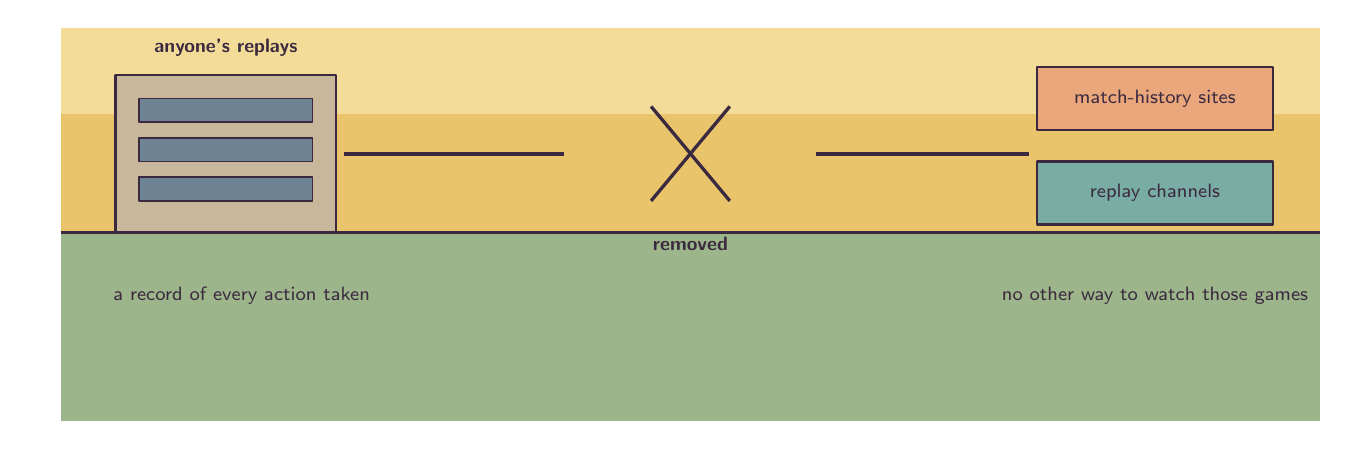
\begin{tikzpicture}[font=\sffamily]
  \fill[sky] (0,2.4) rectangle (16,5.0);
  \fill[skylight] (0,3.9) rectangle (16,5.0);
  \fill[sage] (0,0) rectangle (16,2.4);
  \draw[ln] (0,2.4) -- (16,2.4);
  % The server the replays came from.
  \filldraw[fill=stone, ln] (0.7,2.4) rectangle (3.5,4.4);
  \foreach \y in {2.8,3.3,3.8} \filldraw[fill=slate, thinln] (1.0,\y) rectangle (3.2,\y+0.3);
  \node[tag, text width=3.2cm] at (2.1,4.75) {anyone's replays};
  \node[lab, text width=5.2cm] at (2.3,1.6) {a record of every action taken};
  % The pipe, cut.
  \draw[ln, line width=1.4pt] (3.6,3.4) -- (6.4,3.4);
  \draw[ln, line width=1.4pt] (9.6,3.4) -- (12.3,3.4);
  \draw[ln, line width=1.2pt] (7.5,4.0) -- (8.5,2.8);
  \draw[ln, line width=1.2pt] (8.5,4.0) -- (7.5,2.8);
  \node[tag, text width=3.4cm] at (8.0,2.25) {removed};
  % What was downstream.
  \filldraw[fill=peach, ln] (12.4,3.7) rectangle (15.4,4.5);
  \node[lab, text width=2.8cm] at (13.9,4.1) {match-history sites};
  \filldraw[fill=teal, ln] (12.4,2.5) rectangle (15.4,3.3);
  \node[lab, text width=2.9cm] at (13.9,2.9) {replay channels};
  \node[lab, text width=4.2cm] at (13.9,1.6) {no other way to watch those games};
\end{tikzpicture}
\end{document}
